\subsection{Arc length}

Let $g(t)$ be a function that draws a curve.
The arc length from $g(a)$ to $g(b)$ is given by
$$\int_a^b|g'(t)|\,dt$$
where $|g'(t)|$ is the length of the tangent vector at $g(t)$.
The integral sums over all of the tangent lengths to arrive at the total length
from $a$ to $b$.
For example, let us measure the length of

\medskip
\verb$xrange=(0,1)$

\verb$yrange=(0,1)$

\verb$draw(x^2)$

\begin{center}
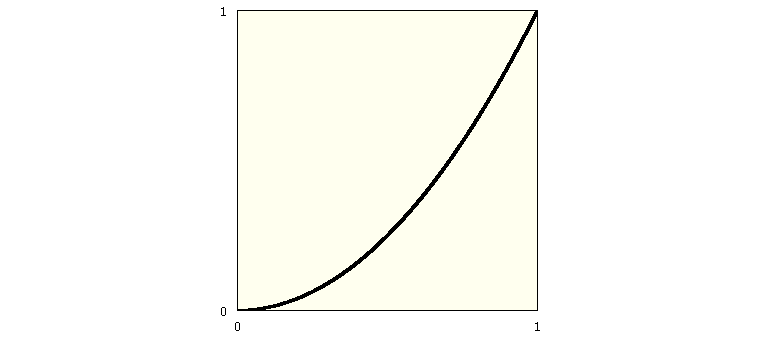
\includegraphics[scale=0.4]{arc.png}
\end{center}

\medskip
\noindent
A suitable $g(t)$ for the arc is
$$g(t)=(t,t^2),\quad0\le t\le1$$
The Eigenmath solution is

\medskip
\verb$g=(t,t^2)$

\verb$defint(abs(d(g,t)),t,0,1)$

$$\hbox{$1\over4$}\log(2+5^{1/2})+\hbox{$1\over2$}5^{1/2}$$

\verb$float$

$$1.47894$$

\medskip
\noindent
As we would expect, the result is greater than $\sqrt2$, the length of the
diagonal.

\medskip
\noindent
The result seems rather complicated given that we
started with a simple parabola.
Let us inspect $|g'(t)|$ to see why.

\medskip
\verb$g$

$$g=\left(\matrix{t\cr t^2}\right)$$

\medskip
\verb$d(g,t)$

$$\left(\matrix{1\cr2t}\right)$$

\medskip
\verb$abs(d(g,t))$

$$(4t^2+1)^{1/2}$$

\medskip
\noindent
The following script does a discrete computation of the arc length by dividing
the curve into 100 pieces.

\medskip
\verb$g(t)=(t,t^2)$

\verb$h(t)=abs(g(t)-g(t-0.01))$

\verb$L=0$

\verb$for(k,1,100,L=L+h(k/100.0))$

\verb$L$

$$L=1.47894$$

\newpage

\subsection{Line integrals}

There are two different kinds of line integrals,
one for scalar fields and one
for vector fields.
The following table shows how both are based on the calculation of
arc length.

\bigskip

\begin{center}
\begin{tabular}{|lll|}
\hline
 & & \\
& Abstract form
& Computable form
\\
 & & \\
Arc length
& $\displaystyle{\int_C ds}$
& $\displaystyle{\int_a^b |g'(t)|\,dt}$
\\
 & & \\
Line integral, scalar field
& $\displaystyle{\int_C f\,ds}$
& $\displaystyle{\int_a^b f(g(t))\,|g'(t)|\,dt}$
\\
 & & \\
Line integral, vector field
& $\displaystyle{\int_C(F\cdot u)\,ds}$
& $\displaystyle{\int_a^b F(g(t))\cdot g'(t)\,dt}$
\\
 & & \\
\hline
\end{tabular}
\end{center}

\bigskip
\noindent
For a vector field, the symbol $u$ is the unit tangent vector
$$u={g'(t)\over|g'(t)|}$$
The length of the tangent vector cancels wth $ds$
as follows.
$$\int_C(F\cdot u)\,ds
=\int_a^b\bigg(F(g(t))\cdot{g'(t)\over|g'(t)|}\bigg)\,\bigg(|g'(t)|\,dt\bigg)
=\int_a^b F(g(t))\cdot g'(t)\,dt
$$

\medskip
\noindent
The following line integral problems are from
{\it Advanced Calculus, Fifth Edition} by Wilfred Kaplan.

\medskip
\noindent
Evaluate $\int y^2\,dx$ along the straight
line from $(0,0)$ to $(2,2)$.

\medskip
\verb$x=2t$

\verb$y=2t$

\verb$g=(x,y)$

\verb$F=(y^2,0)$

\verb$defint(dot(F,d(g,t)),t,0,1)$

$$8\over3$$

\medskip
\noindent
Evaluate $\int z\,dx+x\,dy+y\,dz$
along the path
$x=2t+1$, $y=t^2$, $z=1+t^3$, $0\le t\le 1$.

\medskip
\verb$x=2t+1$

\verb$y=t^2$

\verb$z=1+t^3$

\verb$g=(x,y,z)$

\verb$F=(z,x,y)$

\verb$defint(dot(F,d(g,t)),t,0,1)$

$$163\over30$$

